% Generated from figures/generated/ch08-heads.svg; do not hand edit.
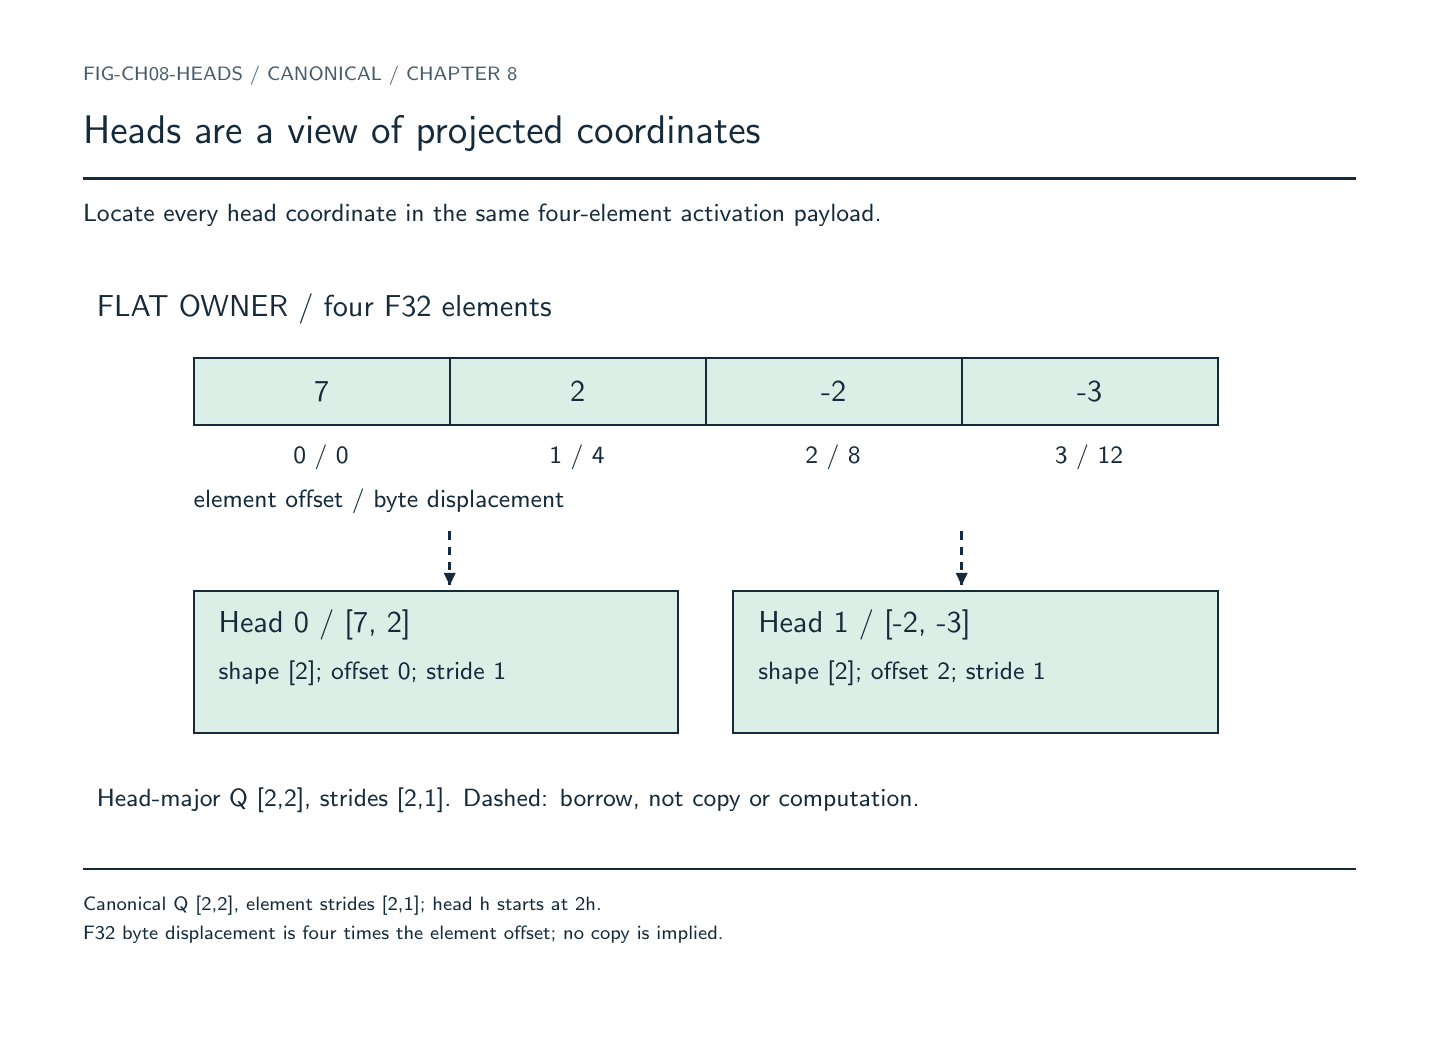
\begin{tikzpicture}[x=.5pt,y=-.5pt]
\path[use as bounding box] (0,0) rectangle (1000,720);
\path[fill=white,draw=none,line width=0.5pt] (0.0,0.0) rectangle (1000.0,720.0);
\node[inner sep=0pt,outer sep=0pt,anchor=base west,text={rgb,255:red,70;green,92;blue,107},font=\sffamily\fontsize{7.0}{8.4}\selectfont] at (40,38) {FIG-CH08-HEADS  /  CANONICAL / CHAPTER 8};
\node[inner sep=0pt,outer sep=0pt,anchor=base west,text={rgb,255:red,21;green,43;blue,60},font=\sffamily\fontsize{15.0}{18.0}\selectfont] at (40,84) {Heads are a view of projected coordinates};
\draw[fill=none,draw={rgb,255:red,21;green,43;blue,60},line width=0.75pt] (40,109) -- (960,109);
\node[inner sep=0pt,outer sep=0pt,anchor=base west,text={rgb,255:red,21;green,43;blue,60},font=\sffamily\fontsize{9.5}{11.4}\selectfont] at (40,140) {Locate every head coordinate in the same four-element activation payload.};
\node[inner sep=0pt,outer sep=0pt,anchor=base west,text={rgb,255:red,21;green,43;blue,60},font=\sffamily\fontsize{10.5}{12.6}\selectfont] at (50,209) {FLAT OWNER / four F32 elements};
\path[fill={rgb,255:red,220;green,239;blue,231},draw={rgb,255:red,21;green,43;blue,60},line width=0.7pt] (120.0,239.0) rectangle (305.0,287.0);
\node[inner sep=0pt,outer sep=0pt,anchor=base west,text={rgb,255:red,21;green,43;blue,60},font=\sffamily\fontsize{9.5}{11.4}\selectfont] at (134,268) {};
\node[inner sep=0pt,outer sep=0pt,anchor=base,text={rgb,255:red,21;green,43;blue,60},font=\sffamily\fontsize{10.5}{12.6}\selectfont] at (212.5,270) {7};
\path[fill={rgb,255:red,220;green,239;blue,231},draw={rgb,255:red,21;green,43;blue,60},line width=0.7pt] (305.0,239.0) rectangle (490.0,287.0);
\node[inner sep=0pt,outer sep=0pt,anchor=base west,text={rgb,255:red,21;green,43;blue,60},font=\sffamily\fontsize{9.5}{11.4}\selectfont] at (319,268) {};
\node[inner sep=0pt,outer sep=0pt,anchor=base,text={rgb,255:red,21;green,43;blue,60},font=\sffamily\fontsize{10.5}{12.6}\selectfont] at (397.5,270) {2};
\path[fill={rgb,255:red,220;green,239;blue,231},draw={rgb,255:red,21;green,43;blue,60},line width=0.7pt] (490.0,239.0) rectangle (675.0,287.0);
\node[inner sep=0pt,outer sep=0pt,anchor=base west,text={rgb,255:red,21;green,43;blue,60},font=\sffamily\fontsize{9.5}{11.4}\selectfont] at (504,268) {};
\node[inner sep=0pt,outer sep=0pt,anchor=base,text={rgb,255:red,21;green,43;blue,60},font=\sffamily\fontsize{10.5}{12.6}\selectfont] at (582.5,270) {-2};
\path[fill={rgb,255:red,220;green,239;blue,231},draw={rgb,255:red,21;green,43;blue,60},line width=0.7pt] (675.0,239.0) rectangle (860.0,287.0);
\node[inner sep=0pt,outer sep=0pt,anchor=base west,text={rgb,255:red,21;green,43;blue,60},font=\sffamily\fontsize{9.5}{11.4}\selectfont] at (689,268) {};
\node[inner sep=0pt,outer sep=0pt,anchor=base,text={rgb,255:red,21;green,43;blue,60},font=\sffamily\fontsize{10.5}{12.6}\selectfont] at (767.5,270) {-3};
\node[inner sep=0pt,outer sep=0pt,anchor=base,text={rgb,255:red,21;green,43;blue,60},font=\sffamily\fontsize{9.5}{11.4}\selectfont] at (212,315) {0 / 0};
\node[inner sep=0pt,outer sep=0pt,anchor=base,text={rgb,255:red,21;green,43;blue,60},font=\sffamily\fontsize{9.5}{11.4}\selectfont] at (397,315) {1 / 4};
\node[inner sep=0pt,outer sep=0pt,anchor=base,text={rgb,255:red,21;green,43;blue,60},font=\sffamily\fontsize{9.5}{11.4}\selectfont] at (582,315) {2 / 8};
\node[inner sep=0pt,outer sep=0pt,anchor=base,text={rgb,255:red,21;green,43;blue,60},font=\sffamily\fontsize{9.5}{11.4}\selectfont] at (767,315) {3 / 12};
\node[inner sep=0pt,outer sep=0pt,anchor=base west,text={rgb,255:red,21;green,43;blue,60},font=\sffamily\fontsize{9.0}{10.799999999999999}\selectfont] at (120,347) {element offset / byte displacement};
\draw[fill=none,draw={rgb,255:red,21;green,43;blue,60},line width=1.25pt,dash pattern=on 3.0pt off 2.5pt] (305,364) -- (305,403);
\path[fill={rgb,255:red,21;green,43;blue,60},draw=none,line width=0.5pt] (305.00,403.00) -- (300.65,394.00) -- (309.35,394.00) -- cycle;
\draw[fill=none,draw={rgb,255:red,21;green,43;blue,60},line width=1.25pt,dash pattern=on 3.0pt off 2.5pt] (675,364) -- (675,403);
\path[fill={rgb,255:red,21;green,43;blue,60},draw=none,line width=0.5pt] (675.00,403.00) -- (670.65,394.00) -- (679.35,394.00) -- cycle;
\path[fill={rgb,255:red,220;green,239;blue,231},draw={rgb,255:red,21;green,43;blue,60},line width=0.7pt] (120.0,407.0) rectangle (470.0,510.0);
\node[inner sep=0pt,outer sep=0pt,anchor=base west,text={rgb,255:red,21;green,43;blue,60},font=\sffamily\fontsize{9.5}{11.4}\selectfont] at (134,436) {};
\node[inner sep=0pt,outer sep=0pt,anchor=base west,text={rgb,255:red,21;green,43;blue,60},font=\sffamily\fontsize{10.5}{12.6}\selectfont] at (138,437) {Head 0 / [7, 2]};
\node[inner sep=0pt,outer sep=0pt,anchor=base west,text={rgb,255:red,21;green,43;blue,60},font=\sffamily\fontsize{9.0}{10.799999999999999}\selectfont] at (138,471) {shape [2]; offset 0; stride 1};
\path[fill={rgb,255:red,220;green,239;blue,231},draw={rgb,255:red,21;green,43;blue,60},line width=0.7pt] (510.0,407.0) rectangle (860.0,510.0);
\node[inner sep=0pt,outer sep=0pt,anchor=base west,text={rgb,255:red,21;green,43;blue,60},font=\sffamily\fontsize{9.5}{11.4}\selectfont] at (524,436) {};
\node[inner sep=0pt,outer sep=0pt,anchor=base west,text={rgb,255:red,21;green,43;blue,60},font=\sffamily\fontsize{10.5}{12.6}\selectfont] at (528,437) {Head 1 / [-2, -3]};
\node[inner sep=0pt,outer sep=0pt,anchor=base west,text={rgb,255:red,21;green,43;blue,60},font=\sffamily\fontsize{9.0}{10.799999999999999}\selectfont] at (528,471) {shape [2]; offset 2; stride 1};
\node[inner sep=0pt,outer sep=0pt,anchor=base west,text={rgb,255:red,21;green,43;blue,60},font=\sffamily\fontsize{9.5}{11.4}\selectfont] at (50,563) {Head-major Q [2,2], strides [2,1]. Dashed: borrow, not copy or computation.};
\draw[fill=none,draw={rgb,255:red,21;green,43;blue,60},line width=0.75pt] (40,608) -- (960,608);
\node[inner sep=0pt,outer sep=0pt,anchor=base west,text={rgb,255:red,21;green,43;blue,60},font=\sffamily\fontsize{7.5}{9.0}\selectfont] at (40,638) {Canonical Q [2,2], element strides [2,1]; head h starts at 2h.};
\node[inner sep=0pt,outer sep=0pt,anchor=base west,text={rgb,255:red,21;green,43;blue,60},font=\sffamily\fontsize{7.5}{9.0}\selectfont] at (40,659) {F32 byte displacement is four times the element offset; no copy is implied.};
\end{tikzpicture}
